\section*{Espacio-tiempo de Schwarzschild \normalfont{\text{$ (a\equiv \frac{2GM}{c^2})$}}}
\begin{align*}
    &\dashv\text{Métrica: } ds^2 = -\left(1-\frac{a}{r}\right)c^2dt^2 + \frac{1}{1-\frac{a}{r}}dr^2 + r^2 d\theta^2 + r^2 \sin^2 \theta d\phi^2 \\
    &\dashv\text{Para cada $t\equiv$ cte, $\theta=\pi/2$: $d\ell^2 = \frac{1}{1-\frac{a}{r}}dr^2 + r^2 d\phi ^2 $}
\end{align*}
\underline{Símbolos de Christoffel (no nulos)}: \text{(símbolos simétricos)}
\begin{align*}
&\begin{cases} 
\Gamma_{01}^0 =\frac{a}{2r(r-a)} \vspace{3pt} \\
\Gamma_{00}^1 = \frac{a}{2r^2}(1-\frac{a}{r})
\vspace{3pt} \\ 
\Gamma_{11}^1 = \frac{a}{2r(a-r)}
\end{cases}
\hspace{-40pt}
&
\begin{cases} 
\Gamma^2_{12}=\frac{1}{r} \vspace{3pt} 
\\ 
\Gamma_{13}^3 =\frac{1}{r}\vspace{3pt}\\ 
\Gamma_{22}^1=a-r
\end{cases} &
\hspace{10pt}
\begin{cases} 
\Gamma^1_{33}=(a-r)\sin^2 \theta \vspace{3pt} \\ 
\Gamma_{33}^2 = -\sin\theta \cos\theta\vspace{3pt}\\ 
\Gamma_{23}^3 = \frac{\cos\theta}{\sin\theta}
\end{cases}  
\end{align*}
\underline{Componentes Tensor de Riemman (no nulos)}:
\begin{align*}
\hspace{-15pt}
&\begin{cases} 
R^0_{\;\;101}=\frac{a}{r(r^2-ar)}
\vspace{2pt}
\\
R^0_{\;\;202}= -\frac{a}{2r}
\vspace{2pt}
\\
R^0_{\;\;303}= -\frac{a\sin^2 \theta}{2r}
\end{cases}
\hspace{-12pt}
&\begin{cases}
R^1_{\; \; 001}= \frac{a(r-a)}{r^4}
\vspace{2pt}
\\
R^1_{\;\;221}=\frac{a}{2r}
\vspace{2pt}
\\
R^1_{\;\;331}= \frac{a\sin^2 \theta}{2r}
\end{cases}
\hspace{-5pt}
&\begin{cases} 
R^2_{\; \; 002}= \frac{a(a-r)}{2r^4}
\vspace{2pt}
\\
R^2_{\;\;121}=\frac{a}{2r^2(a-r)}
\vspace{2pt}
\\
R^2_{\;\;332}=- \frac{a\sin^2 \theta}{r}
\end{cases}
\hspace{-16pt}
&\begin{cases} 
R^3_{\; \; 003}= \frac{a(a-r)}{2r^4}
\vspace{2pt}
\\
R^3_{\;\;131}=\frac{a}{2r^2(a-r)}
\vspace{2pt}
\\
R^3_{\;\;232}= \frac{a}{r}
\end{cases}
\end{align*}
\underline{Paraboloide de Flamm}:\\
\begin{minipage}[c]{0.7\linewidth}
\hspace*{10pt}\vspace*{2pt}
\text{Métrica inducida $\rightarrow$ métrica Schwarzschild ($t\equiv \text{ cte}, \; \theta=\pi/2$)}\\
\hspace*{10pt}\vspace*{2pt}
\text{Visualización de curvatura espacial de métrica Schwarzschild.}\\
\hspace*{10pt}\vspace*{2pt}
\text{No se debe confundir con un pozo de gravedad.}\\
\hspace*{10pt}\vspace*{2pt}
\text{Su ecuación es: $r^2 = \Big(a+\frac{z^2}{4a}\Big)^2.$ Para $z>0$, su representación es: }
\end{minipage}%
\hfill
\begin{minipage}[c]{0.25\linewidth}
    \centering
    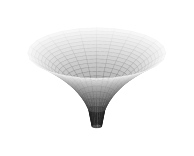
\begin{tikzpicture}[scale=0.35]
      \pgfmathsetmacro{\rs}{0.5}
      \pgfmathsetmacro{\rmax}{7.0}
      \pgfplotsset{colormap={gray}{rgb=(0,0,0) rgb=(0.95,0.95,0.95)}}
      \begin{axis}[
        colormap name=gray,
        view={60}{30},
        axis lines=none,
        domain=0:360, y domain=\rs:\rmax,
        samples=25, samples y=20,
        z buffer=sort
      ]
        \addplot3[surf, shader=flat, opacity=0.6]
          ({y*cos(x)}, {y*sin(x)}, { 2*sqrt(\rs*(y-\rs))});
      \end{axis}
    \end{tikzpicture}
\end{minipage}
\underline{Dilatación gravitacional del tiempo}:
\begin{align*}
    &\text{Relación entre tiempo propio y tiempo coordinado: } \Delta \tau =\sqrt{1-\frac{a}{r}}\;  \Delta t\;  \overset{r\rightarrow\infty}{=}\; \Delta t\\
    &\text{Relación intervalos entre observador a distancia $r$ y observador en $\infty$:}\\
    &T_{\infty}= \frac{1}{\sqrt{1-\frac{a}{r}}}\,T_r \; \Rightarrow\; \text{Redshifting: }   \lambda_{\infty}= \frac{1}{\sqrt{1-\frac{a}{r}}}\,\lambda_r
\end{align*}

